%% LyX 2.3.4.2 created this file.  For more info, see http://www.lyx.org/.
%% Do not edit unless you really know what you are doing.
\documentclass[a4paper,russian]{locconf}
\usepackage[T1,T2A]{fontenc}
\usepackage[utf8]{inputenc}
\usepackage{textcomp}
\usepackage{amsmath}
\usepackage{amssymb}
\usepackage{graphicx}

\makeatletter

%%%%%%%%%%%%%%%%%%%%%%%%%%%%%% LyX specific LaTeX commands.
\pdfpageheight\paperheight
\pdfpagewidth\paperwidth

\DeclareRobustCommand{\cyrtext}{%
  \fontencoding{T2A}\selectfont\def\encodingdefault{T2A}}
\DeclareRobustCommand{\textcyr}[1]{\leavevmode{\cyrtext #1}}


%%%%%%%%%%%%%%%%%%%%%%%%%%%%%% Textclass specific LaTeX commands.
%\usepackage{iopams}
%\usepackage{setstack}

%%%%%%%%%%%%%%%%%%%%%%%%%%%%%% User specified LaTeX commands.
\def\maketitle{}

\makeatother

\usepackage{babel}
\begin{document}
\title{Робастный метод k-means на основе минимизации дифференцируемых оценок
среднего, нечувствительных к~выбросам}
\author{З.М.~Шибзухов$^{1,2}$, М.А.~Казаков$^{1}$, Д.П.~Димитриченко$^{1}$}
\address{$^{1}$Институт прикладной математики и автоматизации -- филиал КБНЦ
РАН, ул.Шортанова 89А, г.\,Нальчик, Россия, 360000.\\
$^{2}$Институт математики и информатики МПГУ, ул. Краснопрудная 14,
г.\,Москва, 107140.}
\begin{abstract}
Предложен новый подход к построению варианта алгоритма кластеризации
\textsf{k-means}, в~котором вместо евклидова расстояния используется
расстояние Махаланобиса. Он основан на~минимизации дифференцируемых
оценок среднего значения, нечувстввительных к~выбросам. На~примерах
показана возможность устойчивости предложенного алгоритма по~отношению
к~выбросам в~данных.
\end{abstract}
\maketitle

\section*{Введение}

Классический метод поиска центров и корреляционных матриц кластеров
представляет решение следующей задачи минимизации:
\begin{equation}
\mathbf{c}_{1}^{*},\dots,\mathbf{c}_{K}^{*}=\arg\min_{\mathbf{c}_{1},\dots,\mathbf{c}_{K}}\frac{1}{N}\sum_{k=1}^{N}\min_{j=1,\dots,K}d(\mathbf{x}_{k};\mathbf{c}_{j},\mathbf{S}_{j}),\label{eq:km_s}
\end{equation}
где $\mathbf{c}_{1},\dots,\mathbf{c}_{K}$~-- центры кластеров,
$\mathbf{S}_{1},\dots,\mathbf{S}_{K}$~-- корреляционные матрицы,
\[
d(\mathbf{x};\mathbf{c},\mathbf{S})=\ln|\mathbf{S}|+(\mathbf{x}-\mathbf{c})^{\prime}\mathbf{S}^{-1}(\mathbf{x}-\mathbf{c})
\]
-- квадрат расстояния Махаланобиса с~корреляционной матрицей $\mathbf{S}$
между точками $\mathbf{x}$~и~$\mathbf{c}$.

Такая постановка задачи основана на~предположении о~том, точки $j$-ого
кластера подчиняются многомерному нормальному распределению с~плотностью
\[
p(\mathbf{x};\mathbf{c},\mathbf{S})\propto\frac{1}{\sqrt{|\mathbf{S}|}}e^{-\frac{1}{2}(\mathbf{x}-\mathbf{c})^{\prime}\mathbf{S}^{-1}(\mathbf{x}-\mathbf{c})},
\]
а произвольная точка $\mathbf{x}$ относится к~кластеру с~номером
\[
j(\mathbf{x})=\arg\max_{j=1,\dots,K}p(\mathbf{x};\mathbf{c}_{j},\mathbf{S}_{j}).
\]

Задача \eqref{eq:km_s} сводится к~решению систем уравнений:
\begin{equation}
\left\{ \begin{array}{l}
\mathbf{c}_{j}={\displaystyle \frac{1}{|\mathbf{I}_{j}|}\sum\limits _{k\in\mathbf{I}_{j}}\mathbf{x}_{k}}\\
\mathbf{S}_{j}={\displaystyle \frac{1}{|\mathbf{I}_{j}|}\sum\limits _{k\in\mathbf{I}_{j}}(\mathbf{x}_{k}-\mathbf{c}_{j})^{\prime}(\mathbf{x}_{k}-\mathbf{c}_{j})},
\end{array}\right.\label{eq:c_S_classic}
\end{equation}
где $\mathbf{I}_{j}\subset\{1,\dots,N\}$~-- индексы точек, попадающих
в~$j$-ый кластер.

Следующая итерационная процедура лежит в~основе алгоритма \textsf{k-means}:
\begin{equation}
\left\{ \begin{array}{l}
\mathbf{c}_{j,t+1}={\displaystyle \frac{1}{|\mathbf{I}_{j,t}|}\sum\limits _{k\in\mathbf{I}_{j,t}}\mathbf{x}_{k}}\\
\mathbf{S}_{j,t+1}={\displaystyle \frac{1}{|\mathbf{I}_{j,t}|}\sum\limits _{k\in\mathbf{I}_{j,t}}(\mathbf{x}_{k}-\mathbf{c}_{j,t})^{\prime}(\mathbf{x}_{k}-\mathbf{c}_{j,t})},
\end{array}\right.\label{eq:kmeans_alg}
\end{equation}
где $\mathbf{I}_{j,t}$~-- индексы точек, попадающих в~$j$-ый
кластер на~$t$-ом шаге. Начальные значения $\mathbf{c}_{1,0},\dots,\mathbf{c}_{K,0}$
и $\mathbf{S}_{1,0},\dots,\mathbf{S}_{K,0}$ задаются перед началом
итерационной процедуры~\eqref{eq:kmeans_alg}.

Существенное искажение результатов работы алгоритма может появиться,
если эмпирическое распределение $\{D(\mathbf{x}_{1}),\dots,D(\mathbf{x}_{N})\}$,
где
\[
D(\mathbf{x})=D(\mathbf{x};\mathbf{c}_{1},\dots,\mathbf{c}_{K};\mathbf{S}_{1},\dots,\mathbf{S}_{K})=\min_{j=1,\dots,K}d(\mathbf{x};\mathbf{c}_{j},\mathbf{S}_{j}),
\]
содержит выбросы.

\section*{Классический метод преодоления влияния выбросов}

Классический метод, направленный на~решение проблемы выбросов, основан
на~замене функции $d(\mathbf{x};\mathbf{c},\mathbf{S})$ на
\[
d_{\varrho}(\mathbf{x};\mathbf{c},\mathbf{S})=\ln|\mathbf{S}|+\varrho\bigl((\mathbf{x}-\mathbf{c})^{\prime}\mathbf{S}^{-1}(\mathbf{x}-\mathbf{c})\bigr),
\]
где $\varrho(r)$~-- функция для подавления влияния выбросов. Она
соответствует вероятностному распределению точек с~плотностью 
\[
p(\mathbf{x};\mathbf{c},\mathbf{S})\propto\frac{1}{\sqrt{|\mathbf{S}|}}e^{-\frac{1}{2}\varrho\bigl((\mathbf{x}-\mathbf{c})^{\prime}\mathbf{S}^{-1}(\mathbf{x}-\mathbf{c})\bigr)}.
\]
 Задача оптимизации имеет вид:
\begin{equation}
\mathbf{c}_{1}^{*},\dots,\mathbf{c}_{K}^{*}=\arg\min_{\mathbf{c}_{1},\dots,\mathbf{c}_{K}}\frac{1}{N}\sum_{k=1}^{N}D_{\varrho}(\mathbf{x}_{k}),\label{eq:km_s_rho}
\end{equation}
где 
\[
D_{\varrho}(\mathbf{x})=D_{\varrho}(\mathbf{x};\mathbf{c}_{1},\dots,\mathbf{c}_{K};\mathbf{S}_{1},\dots,\mathbf{S}_{K})=\min_{j=1,\dots,K}d_{\varrho}(\mathbf{x};\mathbf{c}_{j},\mathbf{S}_{j}).
\]
Введением функции $\varrho$ можно добиться уменьшения \guillemotleft больших\guillemotright{}
значений квадрата функции Махаланобиса, если $\varrho(r)$ растет
не~быстрее, чем линейная. В~качестве примера можно привести функцию
$\varrho(r)=H(\sqrt{r})$, где $H$~-- функция Хьюбера:
\[
H(r)=\begin{cases}
\frac{1}{2}r^{2}, & \text{если}\ r\leqslant c\\
rc-\frac{1}{2}c^{2}, & \text{если}\ r<c.
\end{cases}
\]
Наряду с~функцией Хьюбера можно также использовать функцию $S(r)=\sqrt{c^{2}+r^{2}}-c$,
которая, в~отличие от~нее, имеет непрерывную производную второго
порядка.

Задача \eqref{eq:km_s_rho} сводится к~решению системы уравнений:
\begin{equation}
\left\{ \begin{array}{lc}
\mathbf{c}_{j}=\frac{1}{V_{j}}\sum\limits _{k\in\mathbf{I}_{j}}v_{k}\mathbf{x}_{k}, & V_{j}=\sum\limits _{k\in\mathbf{I}_{j}}v_{k}\\
\mathbf{S}_{j}=\frac{1}{|\mathbf{I}_{j}|}\sum\limits _{k\in\mathbf{I}_{j}}v_{k}(\mathbf{x}_{k}-\mathbf{c}_{j})^{\prime}(\mathbf{x}_{k}-\mathbf{c}_{j}),
\end{array}\right.\label{eq:c_S_rho_eq}
\end{equation}
где $v_{k}=\psi\bigl(D_{\varrho}(\mathbf{x}_{k})\bigr)$, $\psi(r)=\varrho^{\prime}(r)$.

Для единственности решения необходимо, чтобы $\varrho^{\prime}(r)$
была неубывающей. Но из этого вытекает, что достаточно сделать выбросами
порядка $\frac{1}{n+1}$-ой части набора точек, чтобы сломать робастность
такого метода~\cite{Mar1976}. Тем не~менее, если матрицы $\mathbf{S}_{1},\dots,\mathbf{S}_{K}$
заданы, то задача поиска центров $\mathbf{c}_{1},\dots,\mathbf{c}_{K}$
сохраняет робастность. Потеря робастности как раз связана с~оценкой
матриц $\mathbf{S}_{1},\dots,\mathbf{S}_{K}$.

Достаточно содержательный обзор других методов можно найти в~{[}1,2{]}.

\section*{Оценки среднего, нечувствительные к выбросам}

В~настоящей работе предлагается новый подход, основанный на~замене
среднего арифметического в~\eqref{eq:km_s} на~робастную дифференцируемую
оценку среднего $\mathsf{M}\{z_{1},\dots,z_{N}\}$, которая будет
нечувствительной к~выбросам. Такая замена позволит на~уровне математической
постановки задачи заложить фундамент устойчивости решения задачи.

Такие оценки можно построить, как минимум, двумя способами.

\emph{Первый} способ основан приближении медианы на базе $\mathsf{M}$-среднего~{[}3,4{]}
\[
\mathsf{M}_{\rho}\{z_{1},\dots,z_{N}\}=\arg\min_{u}\sum_{k=1}^{N}\rho(z_{k}-u),
\]
где $\rho$ -- дважды дифференцируемая строго выпуклая функция с~минимумом
в~нуле. Определенное таким образом $\mathsf{M}$-среднее имеет частные
производные:
\[
\frac{\partial\mathsf{M}_{\rho}}{\partial z_{k}}=\frac{\rho^{\prime\prime}(z_{k}-\bar{z}_{\rho})}{\rho^{\prime\prime}(z_{1}-\bar{z}_{\rho})+\cdots+\rho^{\prime\prime}(z_{N}-\bar{z}_{\rho})},
\]
где $\bar{z}_{\rho}=\mathsf{M}_{\rho}\{z_{1},\dots,z_{N}\}$. 

Например, если взять функцию $\rho(r)=\sqrt{\varepsilon^{2}+r^{2}}-\varepsilon$,
то при достаточно малых значениях $\varepsilon>0$ можно получить
приближенный и сглаженный вариант медианы. Выбирая достаточно малое
значение $\varepsilon$, можно добиться того, что величина $\rho^{\prime\prime}(z_{k}-\bar{z}_{\rho})=\varepsilon^{2}(\varepsilon^{2}+(z_{k}-\bar{z}_{\rho})^{2})^{-3/2}$
будет пренебрежимо мала для тех значений $z_{k}$, которые находятся
далеко от~среднего значения~$\bar{z}_{\rho}$.

\emph{Второй} способ основан на~применении цензурированного среднего
арифметического, в котором пороговое значение оценивается при помощи
сглаженного варианта $\alpha$-квантиля:
\begin{equation}
\mathsf{WM}_{\rho,\alpha}\{z_{1},\dots,z_{N}\}=\frac{1}{N}\sum_{k=1}^{N}\min\{z_{k},\bar{z}_{\rho_{\alpha},}\},\label{eq:win_mean}
\end{equation}
где $\rho(r)$ -- функция при которой $\mathsf{M}_{\rho}$ выступает
в~качестве приближения медианы,
\begin{equation}
\rho_{\alpha}(r)=\begin{cases}
\alpha\rho(r), & \text{если}\ r>0\\
\frac{1}{2}\bigl(\alpha\rho(0_{+})+(1-\alpha)\rho(0_{+})\bigr), & \text{если}\ r=0\\
(1-\alpha)\rho(r), & \text{если}\ r<0
\end{cases}\label{eq:rho_a}
\end{equation}
является функцией, для которой $\mathsf{M}_{\rho_{\alpha}}\{z_{1},\dots,z_{N}\}$
выступает в~качестве приближения $\alpha$-квантиля. Частные производные
имеют вид:

\[
\frac{\partial\mathsf{WM}_{\rho_{\alpha}}}{\partial z_{k}}=\begin{cases}
\frac{1}{N}+\frac{m}{N}\frac{\partial\mathsf{M}_{\rho_{\alpha}}}{\partial z_{k}}, & \text{если}\ z_{k}<\bar{z}_{\rho_{\alpha}}\\
\frac{m}{N}\frac{\partial\mathsf{M}_{\rho_{\alpha}}}{\partial z_{k}}, & \text{если}\ z_{k}\geqslant\bar{z}_{\rho_{\alpha}},
\end{cases}
\]
где $m$~-- число значений $z_{k}\geqslant\bar{z}_{\rho_{\alpha}}$.
В обоих случаях $\frac{\partial\mathsf{M}}{\partial z_{k}}\geqslant0$
и $\frac{\partial\mathsf{M}}{\partial z_{1}}+\cdots+\frac{\partial\mathsf{M}}{\partial z_{N}}=1$.

Если взять функцию Хьюбера, то можно получить другой вариант: 
\[
\mathsf{M}_{H}\{z_{1},\dots,z_{N}\}=\frac{1}{N-m}\sum_{z_{k}\leqslant c}z_{k}+\frac{m}{N-m}c,
\]
где $m$~-- количество аргументов $z_{k}>c$. Если положим $c=\bar{z}_{\rho_{\alpha}}$,
то
\[
\frac{\partial\mathsf{M}_{H,\rho_{\alpha}}}{\partial z_{k}}=\begin{cases}
\frac{1}{N-m}+\frac{m}{N-m}\frac{\partial\mathsf{M}_{\rho_{\alpha}}}{\partial z_{k}}, & \text{если}\ z_{k}<\bar{z}_{\rho_{\alpha}}\\
\frac{m}{N-m}\frac{\partial\mathsf{M}_{\rho_{\alpha}}}{\partial z_{k}}, & \text{если}\ z_{k}\geqslant\bar{z}_{\rho_{\alpha}}.
\end{cases}
\]
Но при этом, $\frac{\partial\mathsf{M}}{\partial z_{1}}+\cdots+\frac{\partial\mathsf{M}}{\partial z_{N}}=\frac{N}{N-m}$.

\section*{Принцип минимизации дифференцируемых средних, нечувствительных к~выбросам}

Таким образом, в~условиях выбросов, предлагается искать $\mathbf{c}^{*}$
и $\mathbf{S}^{*}$, минимизируя функционал
\[
\mathcal{Q}(\mathbf{c}_{1},...,\mathbf{c}_{K};\mathbf{S}_{1},...,\mathbf{S}_{K})=\mathsf{M}\bigl\{ D(\mathbf{x}_{1};\mathbf{c}_{1},...,\mathbf{c}_{K};\mathbf{S}_{1},...,\mathbf{S}_{K}),\dots,D(\mathbf{x}_{N};\mathbf{c}_{1},...,\mathbf{c}_{K};\mathbf{S}_{1},...,\mathbf{S}_{K})\bigl\}.
\]

В~силу дифференцируемости $\mathsf{M}\{z_{1},\dots,z_{N}\}$ искомые
центры $\mathbf{c}_{1}^{*},\dots,\mathbf{c}_{K}^{*}$ и матрицы $\mathbf{S}_{1}^{*},\dots,\mathbf{S}_{K}^{*}$
являются решением системы нелинейных уравнений:
\begin{equation}
\left\{ \begin{array}{lc}
z_{k}=D(\mathbf{x}_{k};\mathbf{c}_{1},\dots,\mathbf{c}_{K};\mathbf{S}_{1},\dots,\mathbf{S}_{K}), & k=1,\dots,N\\
\mathbf{v}=\nabla\mathsf{M}\{z_{1},\dots,z_{N}\}\\
\mathbf{c}_{j}=\frac{1}{V_{j}}{\displaystyle \sum\limits _{k\in\mathbf{I}_{j}}v_{k}\mathbf{x}_{k}}, & j=1,\dots,K\\
\mathbf{S}_{j}=\frac{1}{V_{j}}{\displaystyle \sum\limits _{k\in\mathbf{I}_{j}}v_{k}(\mathbf{x}_{k}-\mathbf{c}_{j})^{\prime}(\mathbf{x}_{k}-\mathbf{c}_{j})}, & j=1,\dots,K
\end{array}\right.\label{eq:eq_c_S}
\end{equation}

Вектор весов $\mathbf{v}$ при $\mathbf{c}_{j}=\mathbf{c}_{j}^{*}$
и $\mathbf{S}_{j}=\mathbf{S}_{j}^{*}$ также можно использовать в~качестве
оценки значимости точек. Так как $v_{1}+\cdots+v_{N}=1$, то выбросам
будут соответствовать точки с~наименьшими значениями весов.

Устойчивость по~отношению к~выбросам достигается за~счет того,
что веса точек, соответствующих выбросам, оказывается существенно
меньше, чем веса точек, не~являющихся выбросами. Важно также то,
величина веса точки убывает по~мере роста модуля разности между $\bar{z}=\nabla\mathsf{M}\{z_{1},\dots,z_{N}\}$
и $z_{k}$. Такие свойства являются естественным следствием робастности
оценок среднего значения. 

Например, для $\mathsf{M}_{\rho}\{z_{1},\dots,z_{N}\}$
\[
v_{k}=\frac{\rho^{\prime\prime}(z_{k}-\bar{z}_{\rho})}{\rho^{\prime\prime}(z_{1}-\bar{z}_{\rho})+\cdots+\rho^{\prime\prime}(z_{N}-\bar{z}_{\rho})}.
\]
При $\rho(r)=\sqrt{\varepsilon^{2}+r^{2}}-\varepsilon$ 
\[
v_{k}<\left(\frac{\varepsilon^{2}+(z_{k}-\bar{z}_{\rho})^{2}}{\varepsilon^{2}+(z_{(1)}-\bar{z}_{\rho})^{2}}\right)^{3/2},
\]
где $z_{(1)}$ -- ближайшее значение к~$\bar{z}_{\rho}$. Так что,
$v_{k}$, будучи заключено между $0$ и $1$, быстро убывает по~мере
его удаления от~$\bar{z}_{\rho}$. 

Для $\mathsf{WM}_{\rho}\{z_{1},\dots,z_{N}\}$, соответственно, получаем
\[
\begin{cases}
\frac{1}{N}\leqslant v_{k}<\frac{1}{N}+\frac{m}{N}\left(\frac{\varepsilon^{2}+(z_{k}-\bar{z}_{\rho})^{2}}{\varepsilon^{2}+(z_{(1)}-\bar{z}_{\rho})^{2}}\right)^{3/2}, & \text{если}\ z_{k}<\bar{z}_{\rho}\\
v_{k}<\frac{m}{N}\left(\frac{\varepsilon^{2}+(z_{k}-\bar{z}_{\rho})^{2}}{\varepsilon^{2}+(z_{(1)}-\bar{z}_{\rho})^{2}}\right)^{3/2}, & \text{если}\ z_{k}\geqslant\bar{z}_{\rho}.
\end{cases}
\]
Здесь при $z_{k}\geqslant\bar{z}_{\rho}$ вес $v_{k}$ быстро падает
по~мере удаления от~$\bar{z}_{\rho}$. Веса $v_{k}>1/N$ при $z_{k}<\bar{z}_{\rho}$
и быстро приближаются к~$1/N$ по~мере удаления значения $z_{k}$
от~$\bar{z}_{\rho}$.

\begin{figure}
\noindent 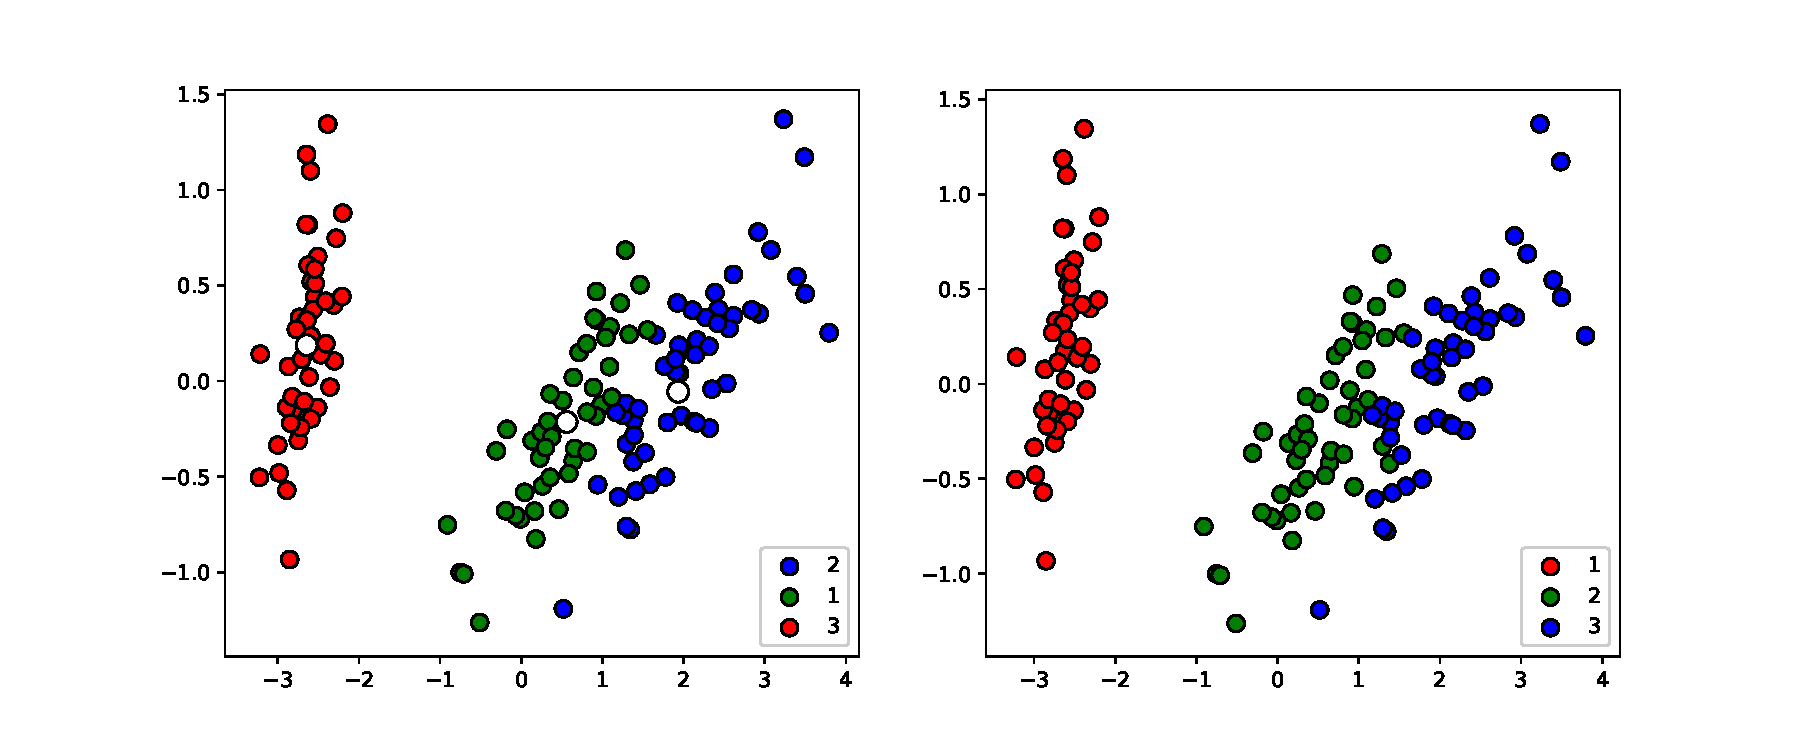
\includegraphics[width=0.9\textwidth]{kmeans_iris2_robust}

\noindent \hspace*{\fill}а)\hspace*{\fill}б)\hspace*{\fill}
\noindent \centering{}\caption{\textsf{IRIS}: Робастный алгоритм}
\end{figure}

\begin{figure}
\noindent 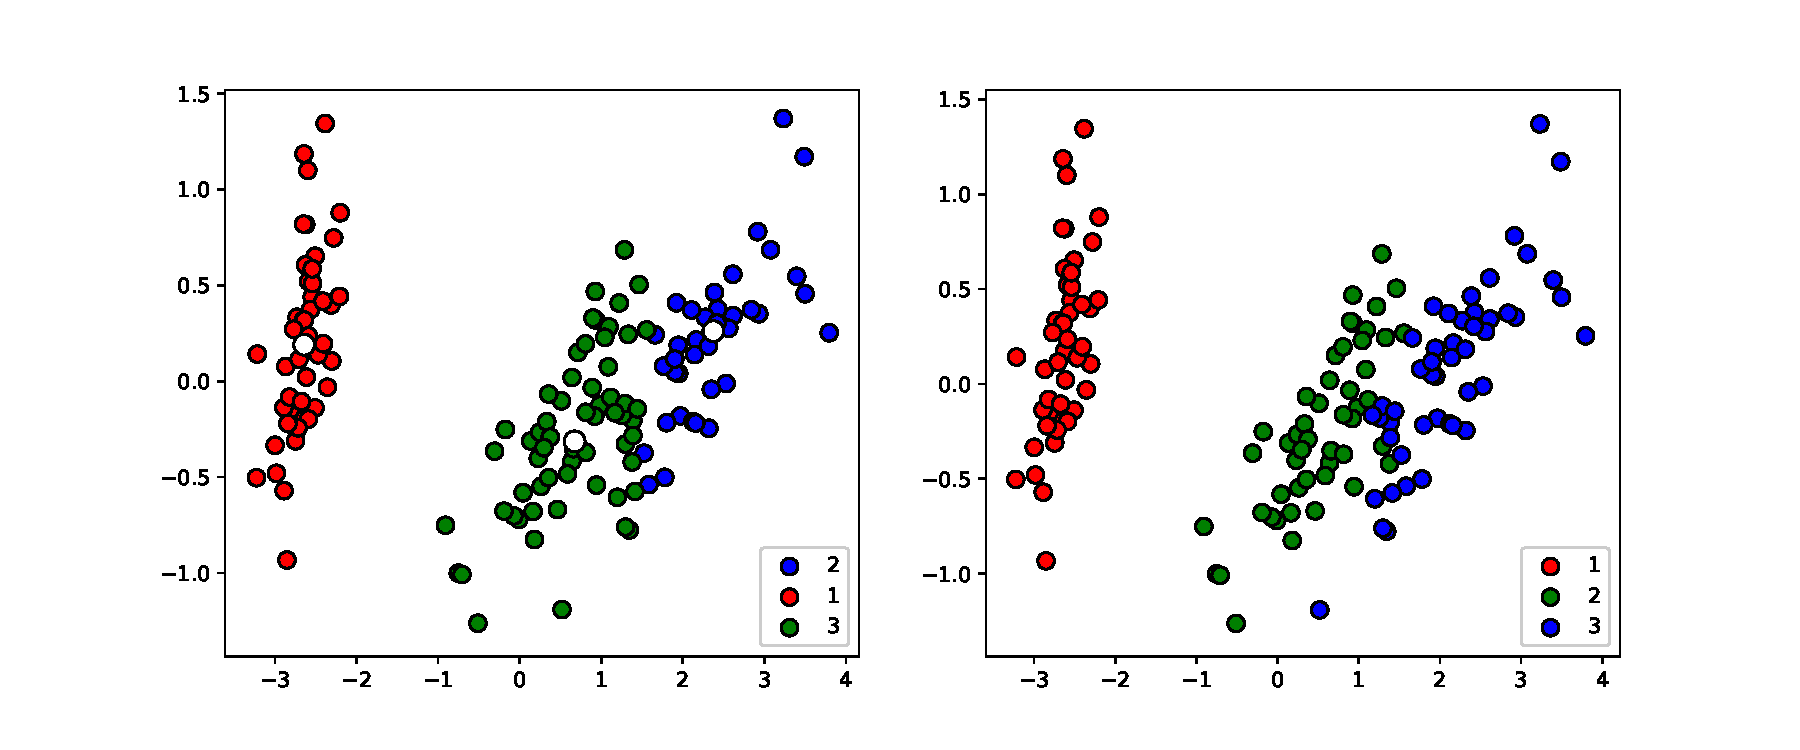
\includegraphics[width=0.9\textwidth]{kmeans_iris2_kmeans}

\noindent \hspace*{\fill}а)\hspace*{\fill}б)\hspace*{\fill}

\noindent \caption{\textsf{IRIS}: Классический алгоритм.}
\end{figure}


\section*{Алгоритм}

Для поиска $\mathbf{c}_{1}^{*},\dots,\mathbf{c}_{K}^{*}$ и $\mathbf{S}_{1}^{*},\dots,\mathbf{S}_{K}^{*}$
применим итерационную схему, которая соответствует аналогу методу
Якоби для решения системы нелинейных уравнений~\eqref{eq:eq_c_S}.

Начальные положения центров выбираются некоторым образом, например:
\[
\left\{ \begin{array}{l}
\mathbf{c}_{j,0}={\displaystyle \frac{1}{N}\sum\limits _{k=1}^{N}\mathbf{x}_{k}}\\
\mathbf{S}_{j,0}=\mathbf{E}^{n\times n},
\end{array}\right.
\]
где $\mathbf{E}^{n\times n}$~-- единичная матрица $n\times n$.
\begin{enumerate}
\item На $t$-ом шаге последовательно решаются два уравнения:
\begin{enumerate}
\item Для каждого $j=1,\dots,K$ сначала решается следующее векторное уравнение
для нахождения $\mathbf{c}_{j,t+1}$:
\begin{equation}
\mathbf{c}_{j}=\sum\limits _{k\in\mathbf{I}_{j}}\frac{\partial\mathsf{M}\{z_{1},\dots,z_{N}\}}{\partial z_{k}}\mathbf{x}_{k},\label{eq:eq_c}
\end{equation}
где $z_{k}=D(\mathbf{x}_{k};\mathbf{c}_{1},\dots,\mathbf{c}_{K};\mathbf{S}_{1,t},\dots,\mathbf{S}_{K,t})$.
\item Затем для каждого $j=1,\dots,K$ решается следующее векторное уравнение
для нахождения $\mathbf{S}_{j,t+1}$:
\begin{equation}
\mathbf{S}_{j}=\sum\limits _{k\in\mathbf{I}_{j}}\frac{\partial\mathsf{M}\{z_{1},\dots,z_{N}\}}{\partial z_{k}}(\mathbf{x}_{k}-\mathbf{c}_{j,t+1})^{\prime}(\mathbf{x}_{k}-\mathbf{c}_{j,t+1}),\label{eq:eq_S}
\end{equation}
где $z_{k}=D(\mathbf{x}_{k};\mathbf{c}_{t+1},\mathbf{S})$.
\end{enumerate}
\item Шаг 1 повторяется до тех пор, пока $t<T$ (максимальное число итераций)
или последовательность $\{\mathcal{Q}(\mathbf{c}_{t,1},\dots,\mathbf{c}_{t,K};\mathbf{S}_{t,1},\dots,\mathbf{S}_{t,K})\}$
не~сконцентрируется вокруг своей точки сгущения.
\end{enumerate}
Множества индексов точек $\mathbf{I}_{1},\dots,\mathbf{I}_{K}$, соответствующие
разбиению на~кластеры, находятся перед решением систем уравнений.
Дополнительное условие $|\mathbf{S}|=1$ обычно добавляется, чтобы
предотвратить вырождение корреляционной матрицы. Показатель масштаба
$\sigma=|\mathbf{S}|$ можно затем оценить при помощи $\mathsf{S}$-эстиматора~\cite{Dav1987}.

Первое уравнение в системе имеет вид:
\[
\mathbf{c}=F(\mathbf{c}).
\]
Для его решения можно использовать итерационную процедуру:
\[
\mathbf{c}_{t+1}=(1-h)\mathbf{c}_{t}+hF(\mathbf{c}_{t}),
\]
где $0\leqslant h\leqslant1.$ Второе уравнение имеет аналогичный
вид:
\[
\mathbf{S}=G(\mathbf{S}).
\]
Для его решения можно использовать аналогичную итерационную процедуру:
\[
\mathbf{S}_{t+1}=(1-h)\mathbf{S}_{t}+hG(\mathbf{S}_{t}),
\]


\section*{Примеры}

\begin{figure}
\noindent 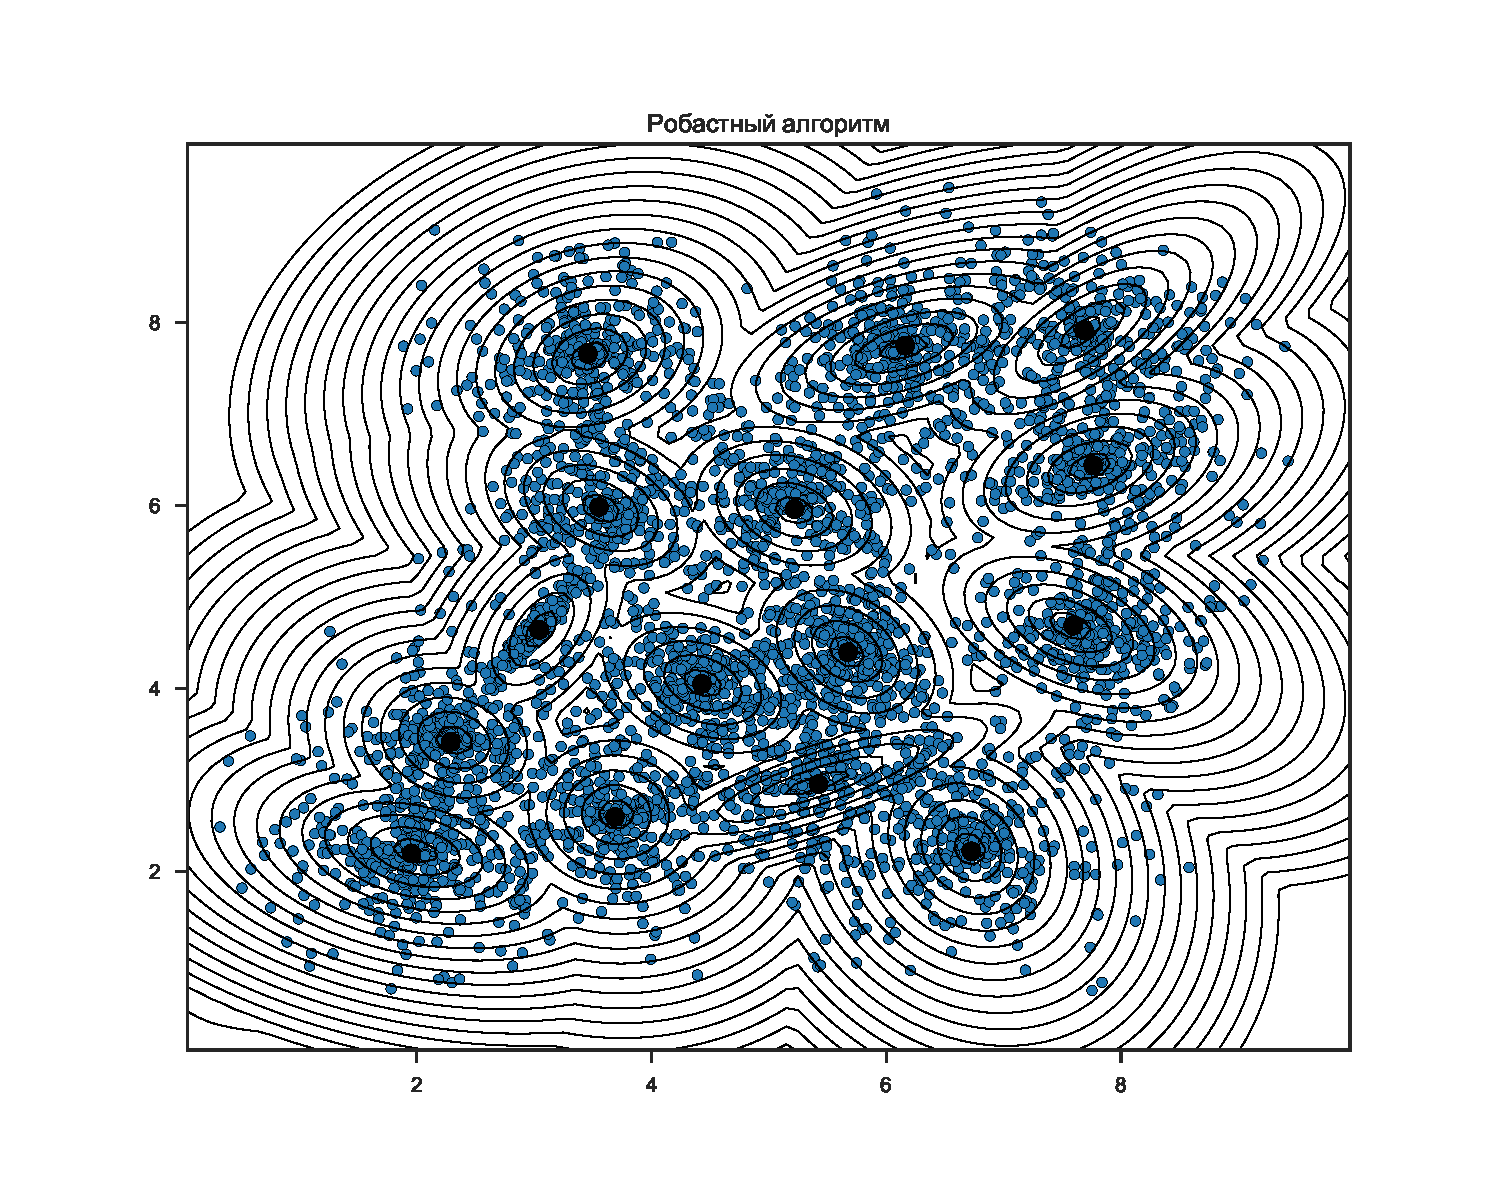
\includegraphics[width=0.5\textwidth]{kmeans_s3_robust}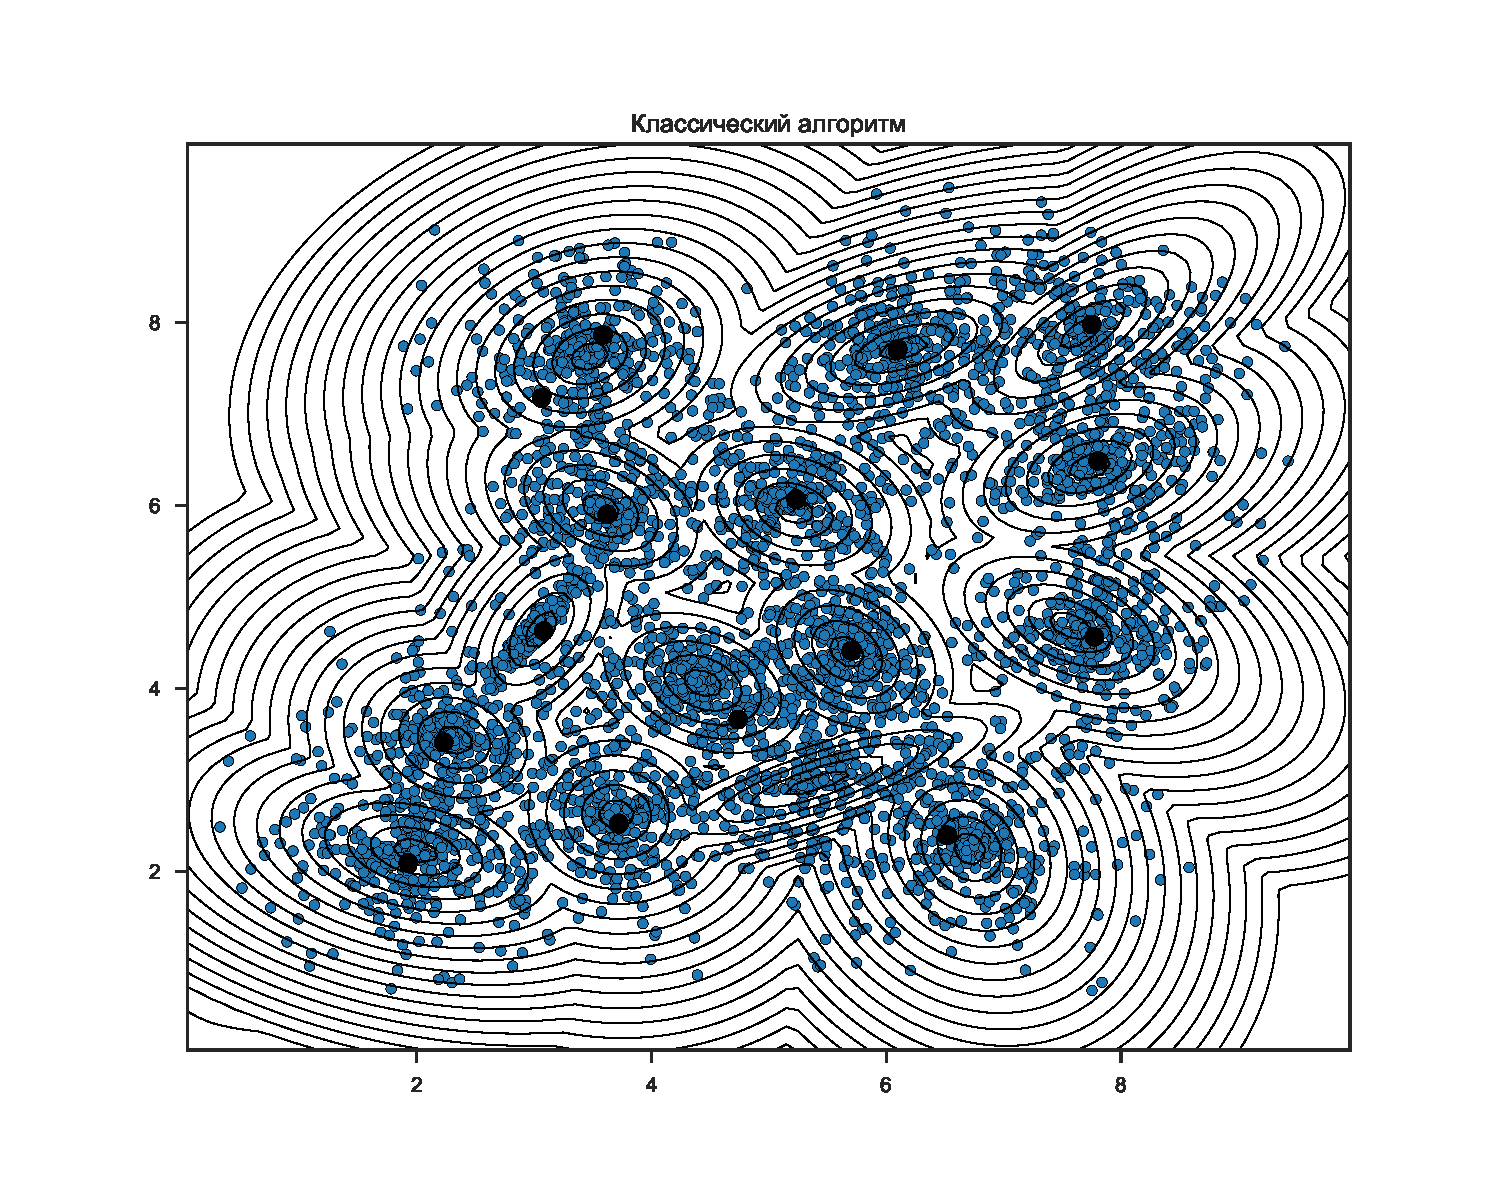
\includegraphics[width=0.5\textwidth]{kmeans_s3_kmeans}

\noindent \hspace*{\fill}а)\hspace*{\fill}\hspace*{\fill}б)\hspace*{\fill}
\noindent \centering{}\caption{\textsf{S3}: Результаты робастного и классического алгоритмов.}
\end{figure}

\begin{figure}
\noindent 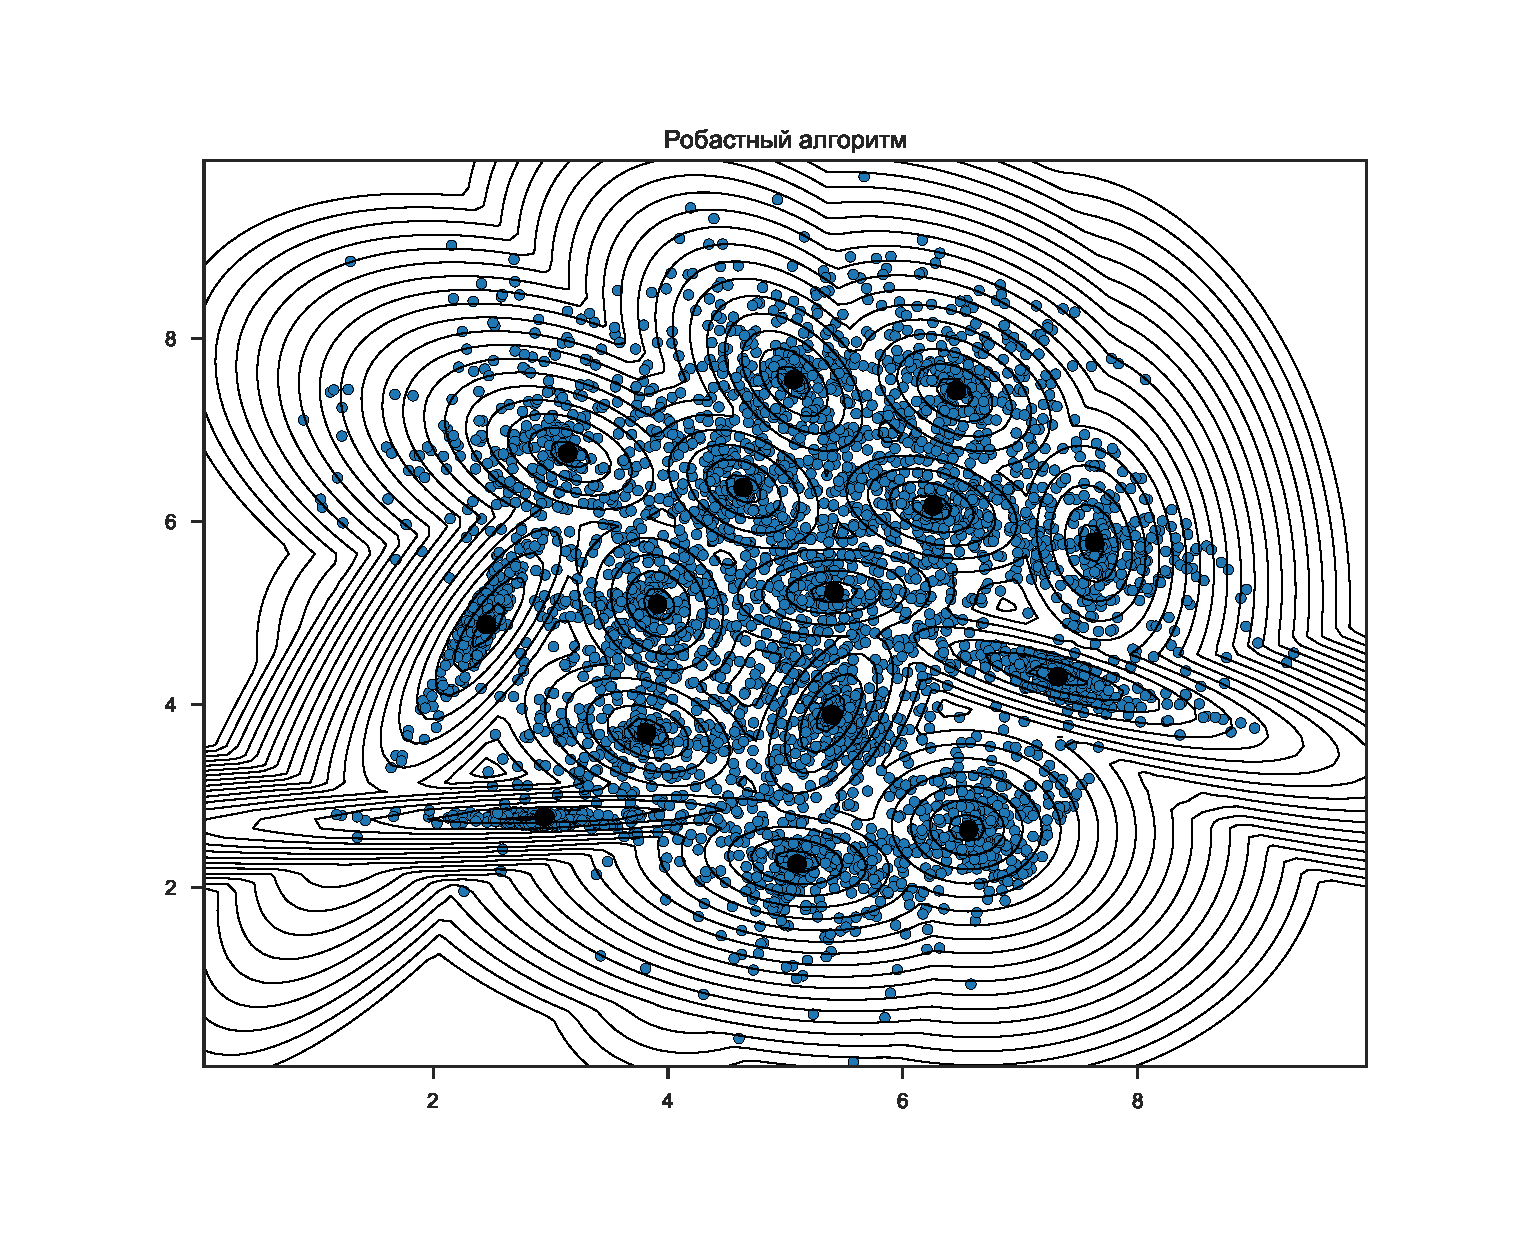
\includegraphics[width=0.5\textwidth]{kmeans_s4_robust}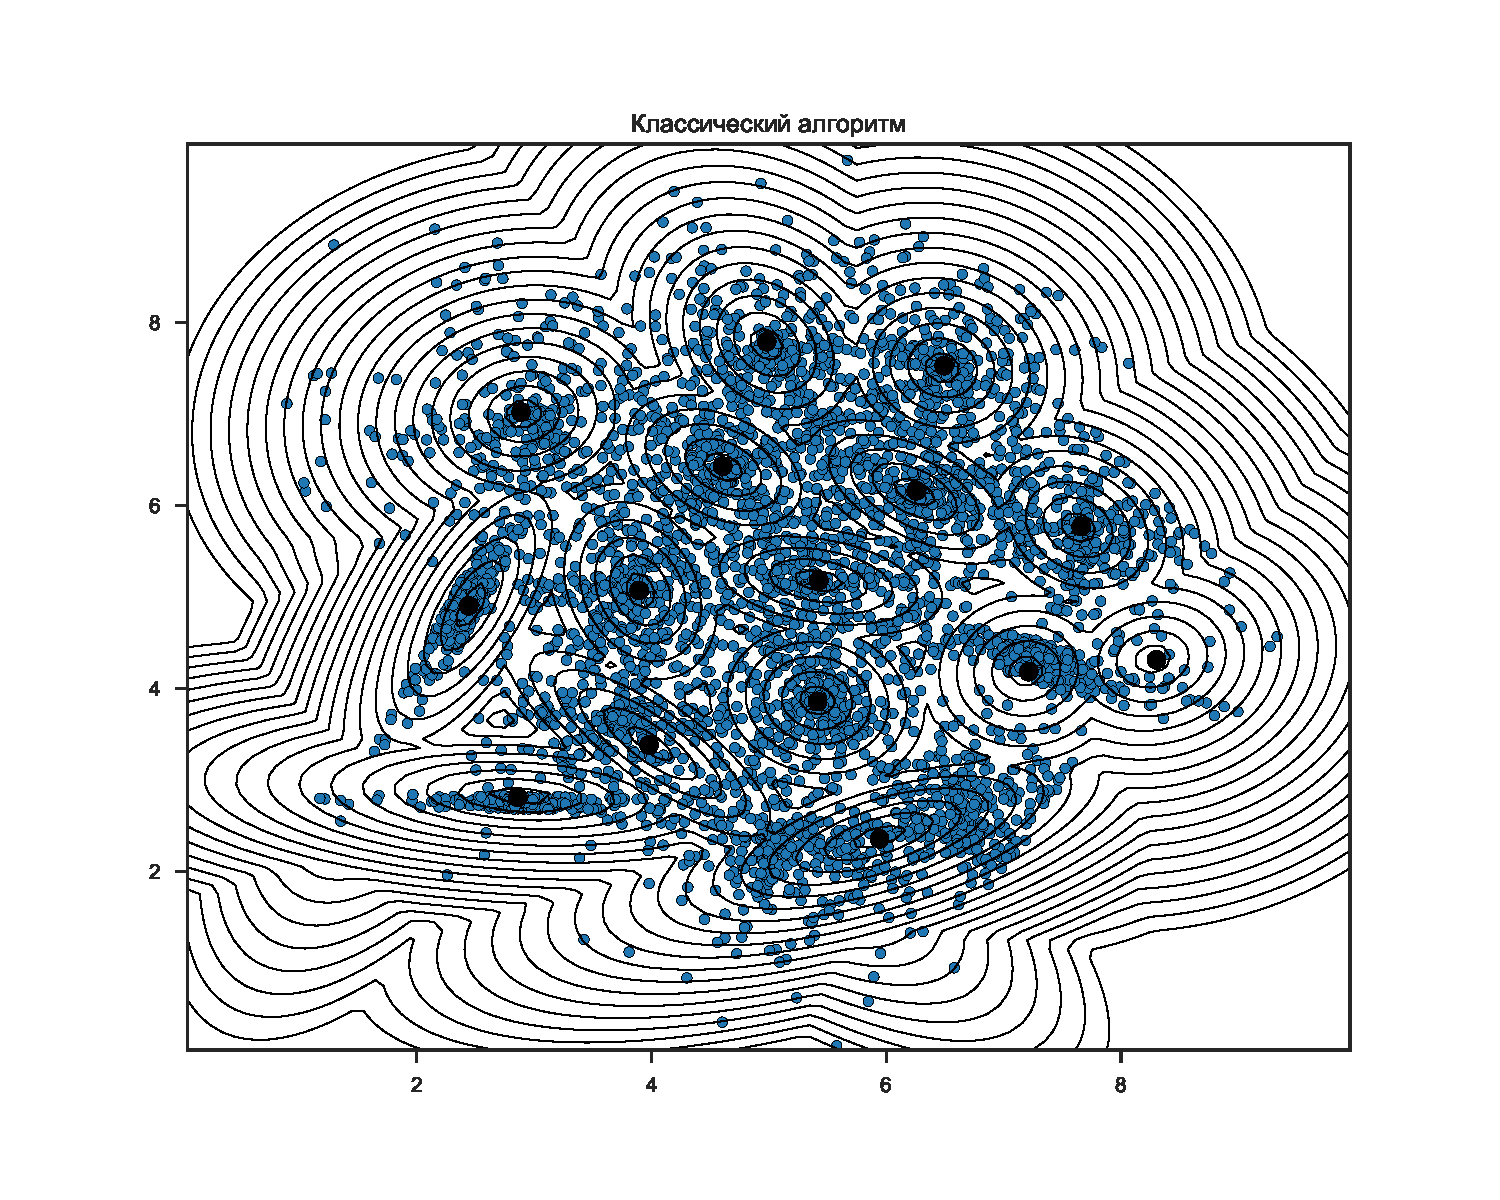
\includegraphics[width=0.5\textwidth]{kmeans_s4_kmeans}

\noindent \hspace*{\fill}а)\hspace*{\fill}\hspace*{\fill}б)\hspace*{\fill}\caption{\textsf{S4}: Результаты робастного и классического алгоритмов.}
\end{figure}

\textbf{1.} Расмотрим относительно простой и классический набор данных
\textsf{iris}. Как правило, он используется для задач классификации.
Мы же здесь попытаемся идентифицировать классы при помощи кластеризации,
используя расстояния Махаланобиса вместо Евклидового. На Рис.~1 слева
на~а) представлен результат робастной кластеризации, справа на~б)
исходное разбиение на~классы. Нетрудно убедиться, что можно получить
разбиение, которое отличается от~заданного в~3-х точках из~150-ти.
Для сравнение на Рис.~2 приведено разбиение, полученное при помощи
классического метода. Здесь отличие в~5-ти точках. Хотя прееимущество
минимальное, но с~учетом того, что наилучшие надежные алгоритмы классификации
по~данным набора iris как раз дают 98\% точности и выше, то это можно
считать хорошим результатом. Он показывает, что применение робастного
подхода к~кластеризации на~основе реалистичного набора признаков
можно получать разбиения, которые практически соответствуют заданной
классификации.

\textbf{2.} Рассмотрим наборы данных \textsf{S3-S4}~из~\cite{SD2018,sdataset}.
Они содержит 5000 точек, 15 кластеров. Среди наборов данных \textsf{S1--S4}~\cite{sdataset},
в \textsf{S3-S4} доля выбросов -- \emph{наибольшая}. Именно поэтому
этот набор данных представляет наибольший интерес. Для сравнения приведем
результаты применения стандартный метода \textsf{k-means}, но с учетом
корреляционной матрицы. На Рис.~3~и ~4 представлены результаты
кластеризации для наборов \textsf{S3} и \textsf{S4}, соответственно.
На~а) представлен результат работы робастного алгоритма, а на~б)
-- классического.

\section*{Заключение}

В настоящей работе рассмотривался вариант \textsf{k-means}, в~котором
вместо евклидова расстояния использовалось расстояние Махаланобиса.
Предложенный новый подход к~построению робастного варианта \textsf{k-means}
на~основе расстояния Махаланобиса, основанный на минимизации робастных
дифференцируемых оценок среднего показал свою принципиальную устойчивость
к~искажениям в~данных, по~сравнению с~классическим алгоритмом
\textsf{k-means}. Связано это с~тем, что применяемые в~работе робастные
оценки среднего ограничивают влияние на~поиск положения центров кластеров
точек, которые расположены на~относительно больших расстояниях от~них.

\section*{Благодарности}

Работа выполнена при поддержке гранта РФФИ №18--01--00050.

\section*{Литература}
\begin{thebibliography}{1}
\bibitem{Mar1976}Maronna~R.A. Robust M-Estimators of Multivariate
Location and Scatter / R.A.~Maronna // Ann. Statist, 1976 -- Vol.4
-- PP.51--67. 

\bibitem{RH2013}Rousseeuw~P. High-breakdown estimators of multivariate
location and scatter / P.~Rousseeuw, M.\textasciitilde Hubert //
Robustness and Complex Data Structures. Ed.: C.~Becker, R.~Fried,
S.~Kuhnt., 2013 -- Springer -- PP.~49--66.

\bibitem{MY}Maronna~R.A. Robust and efficient estimation of multivariate
scatter and location / R.A.~Maronna, V.J.~Yohai // arxiv:1504.03389,
2015.

\bibitem{SZ2017dan}Шибзухов~З.М. О принципе минимизации эмпирического
риска на основе усредняющих агрегирующих функций / \emph{З.М.~Шибзухов}
// Доклады РАН. М.:МАИК \guillemotleft Наука\guillemotright , 2017
-- Т.476 -- №5 -- С.495-499.

\bibitem{SZK2019itnt}Shibzukhov~Z.M. Clustering based on the principle
of finding centers and robust averaging functions of aggregation /
Z.M.~Shibzukhov, M.A.~Kazakov // Proceedings of V International
Conference Information Technology and Nanotechnology -- ITNT 2019.
Journal of Physics: Conference Series {[}Электронный ресурс{]} --
Режим доступа: https://iopscience.iop.org/article/10.1088/1742-6596/1368/5/052010/pdf

\bibitem{Dav1987}Davies~P.L. Asymptotic behavior of S-estimates
of multivariate location parameters and dispersion matrices / P.L.~Davies
// Ann. Statist. -- 1987 -- Vol.15 -- PP.1269--1292.

\bibitem{SD2018}Fränti~P. , Sieranoja~S. K-means properties on
six clustering benchmark datasets / P.~Fränti, S.~Sieranoja // Applied
Intelligence -- 2018 -- V.48 -- No.12 -- PP.4743--4759.

\bibitem{sdataset} Clustering basic benchmark {[}Электронный ресурс{]}.
-- Режим доступа: http://cs.joensuu.fi/sipu/datasets/
\end{thebibliography}
\newpage{}

\smallskip
\noindent{\Large\bf{Robust k-means method based on~minimizing \\ differentiable estimates of~mean insensitive to~outliers}}

\vspace{0.5cm}
\hangindent=2.5cm \noindent \hangafter=-1 {\bf $^{1,2}$\,Z.M.~Shibzukhov, $^1$\,M.A.~Kazakov, $^2$\,D.P.~Dimitrichenko}

\vspace{0.5cm}
\hangindent=2.5cm \noindent \hangafter=-2 {$^1$\,Institute of Applied Mathematics and Automation KBSC RAS, Shortanova st.89A, Nalchick, Russia}

\hangindent=2.5cm \noindent \hangafter=-2 {$^2$\,Institute of mathematics and Informatics MPSU, Krasnoprudnaya st. 14, Moscow, Russia}

\vspace{1cm}
\hangindent=2.5cm \noindent \hangafter=-5 {\bf Abstract.} A new approach toconstructing avariant of the k-means clustering algorithm isproposed, in which the Mahalanobis distance is used instead of the Euclidean distance. It is based on minimizing differentiable estimates of average values that are insensitive tooutliers. The examples show the possibility of stability of the proposed algorithm with respect tooutliers in the data.

\end{document}
